\subsection{Words, dwell times, and closure}
\label{subsec:generalized-reeb-orbits-polytopes-words}

The finite computation records a simple orbit by its facet directions, dwell
times, and starting point. We use the \emph{active-word convention}: the word
contains exactly the distinct facet directions that occur with positive
duration, and the base point is chosen at a velocity breakpoint. A cyclic word
\[
  \sigma=(\sigma_1,\ldots,\sigma_m)
\]
with distinct entries, together with dwell times \(\tau_k>0\) and a base point
\(b=\gamma(0)\), describes the velocity data
\[
  \dot{\gamma}(t)=R_{\sigma_k}
  \quad\text{for a time interval of length }\tau_k.
\]
Such data can represent a closed orbit only if the closing equation holds:
\begin{equation}\label{eq:generalized-reeb-closure}
  \sum_{k=1}^m \tau_k R_{\sigma_k}=0.
\end{equation}
Closure of the velocity polygon is only the closedness equation for the broken
path. To turn the word and dwell times into an actual simple Reeb orbit on
\(\partial K\), one must choose a base point \(b\) so that each segment lies on
its prescribed facet; this is the base-point recovery construction of
Lemma~\ref{lem:generalized-reeb-base-point-recovery}.

\begin{figure}[htbp]
  \centering
  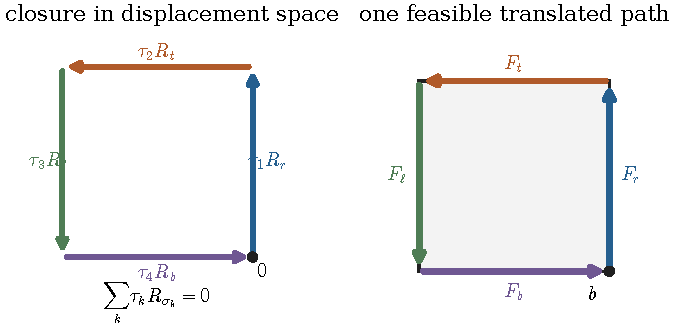
\includegraphics[width=0.94\linewidth]
    {figures/foundations/word-closure-basepoint.pdf}
  \caption{The two layers of finite orbit data in a two-dimensional
  Hamiltonian analogue.  The ordered displacements first form a closed
  velocity polygon.  A translation by a feasible base point then places every
  segment on its prescribed facet.  This is an exact planar example, not a
  projection of the four-dimensional orbit; it illustrates only closure and
  facet realizability.}
  \label{fig:generalized-reeb-word-closure-basepoint}
\end{figure}

Closure does not imply that the second layer is feasible.  For example, in the
planar square \([-1,1]^2\), the right and left facet rows give opposite
directions \(R_r=(0,2)\) and \(R_\ell=(0,-2)\).  Equal dwell times satisfy
\(\tau R_r+\tau R_\ell=0\), but the breakpoint between the two segments would
have to lie in the disjoint facets \(F_r\) and \(F_\ell\).  No translation can
realize this closed two-segment path on the prescribed facets.

The period and action of a closed pure-word orbit are
\[
  T=\sum_{k=1}^m \tau_k,
  \qquad
  A(\gamma)=T.
\]
This convention is the free-period convention used in
Theorem~\ref{thm:preliminaries-clarke-dual-action}.

The same geometric orbit has no preferred starting segment. Cyclically shifting
the \((\text{facet},\text{duration})\)-pairs gives the same orbit, provided the
base point is shifted to the corresponding breakpoint on the curve. If an orbit
is instead started inside a constant-velocity segment, that segment is split at
the start time and then merged again when the active word is recovered. If one
uses a padded convention with all facets in a permutation and dwell times
\(\tau_k\geq0\), then zero-duration entries are first deleted to recover the
active word.

The action of a finite word can be calculated directly from its velocities and
dwell times.

\begin{lemma}[Symplectic shoelace formula]\label{lem:preliminaries-shoelace}
Let \(z\colon[0,T]\to\mathbb{R}^4\) be a closed piecewise affine curve. Suppose
that \(z\) has constant velocity \(w_k\) on consecutive intervals of length
\(\ell_k\), for \(k=1,\ldots,m\). Then
\begin{equation}\label{eq:preliminaries-shoelace}
  2A(z)
  =
  \sum_{1\leq j<k\leq m}
    \ell_j\ell_k\,\omega_0(w_j,w_k).
\end{equation}
In particular, the action of a closed pure-word Reeb orbit depends only on the
cyclic velocity word and the dwell times, not on the base point.
\end{lemma}

\begin{proof}
Write \(t_k=\sum_{j<k}\ell_j\). On the \(k\)-th interval,
\[
  z(t)=z(0)+\sum_{j<k}\ell_jw_j+(t-t_k)w_k.
\]
The contribution of \(z(0)\) to
\(\int_0^T\langle -J_0\dot z,z\rangle\,dt\) vanishes because \(z\) is closed,
so \(\sum_k\ell_kw_k=0\). The self-term
\(\langle -J_0w_k,w_k\rangle\) vanishes by skew-symmetry. Hence
\[
  2A(z)
  =
  \sum_k
    \ell_k\left\langle -J_0w_k,\sum_{j<k}\ell_jw_j\right\rangle
  =
  \sum_{j<k}\ell_j\ell_k\,\omega_0(w_j,w_k),
\]
using \(\omega_0(u,v)=\langle J_0u,v\rangle\).
\end{proof}

Breakpoints of \(\dot{\gamma}\) are velocity changes, not necessarily changes
in the minimal face containing \(\gamma(t)\): an orbit may move inside a
nonsmooth face while switching from one active facet direction to another.

\begin{lemma}[Base-point recovery]\label{lem:generalized-reeb-base-point-recovery}
Fix an active word \(\sigma=(\sigma_1,\ldots,\sigma_m)\) and dwell times
\(\tau_k>0\) satisfying the closure equation
\eqref{eq:generalized-reeb-closure}. Put
\[
  v_1=0,
  \qquad
  v_k=\sum_{j=1}^{k-1}\tau_jR_{\sigma_j}
  \quad (k=2,\ldots,m+1).
\]
Then \(v_{m+1}=0\). A point \(b\in\mathbb{R}^4\) recovers a simple Reeb orbit
with these velocity data, by
\[
  \gamma(t)=b+v_k+sR_{\sigma_k},
  \qquad 0\leq s\leq \tau_k
\]
on the \(k\)-th segment, if and only if
\begin{equation}\label{eq:generalized-reeb-base-point-equalities}
  \langle a_{\sigma_k}, b+v_k\rangle=1
  \quad\text{for }k=1,\ldots,m,
\end{equation}
and
\begin{equation}\label{eq:generalized-reeb-base-point-inequalities}
  \langle a_i,b+v_k\rangle\leq 1
  \quad\text{for }i=1,\ldots,F\text{ and }k=1,\ldots,m.
\end{equation}
Equivalently, the equalities have the form
\[
  N_\sigma b = r_\sigma,
  \qquad
  (N_\sigma)_{k\bullet}=a_{\sigma_k}^{\mathsf T},
  \qquad
  (r_\sigma)_k=1-\langle a_{\sigma_k},v_k\rangle .
\]
When this system is nonempty, its solution space is an affine space of
dimension \(4-\operatorname{rank}N_\sigma\). The inequalities cut out the
valid base points as a convex polytope inside this affine space. In particular,
the set of valid base points is bounded, because \(v_1=0\) and
\eqref{eq:generalized-reeb-base-point-inequalities} imply \(b\in K\).
\end{lemma}

\begin{proof}
On the \(k\)-th segment, the prescribed facet equation is
\[
  \langle a_{\sigma_k}, b+v_k+sR_{\sigma_k}\rangle=1.
\]
The \(s\)-term vanishes because
\(\langle a_{\sigma_k},R_{\sigma_k}\rangle
=2\langle a_{\sigma_k},J_0a_{\sigma_k}\rangle=0\). Hence the whole segment
lies on \(F_{\sigma_k}\) exactly when
\eqref{eq:generalized-reeb-base-point-equalities} holds.

The segment lies in \(K\) exactly when
\[
  \langle a_i,b+v_k+sR_{\sigma_k}\rangle\leq 1
  \quad\text{for all }i\text{ and all }s\in[0,\tau_k].
\]
For fixed \(i,k\) this expression is affine in \(s\), so it is enough to check
the endpoints. The endpoint at \(s=0\) is \(b+v_k\), and the endpoint at
\(s=\tau_k\) is \(b+v_{k+1}\). As \(k\) runs cyclically and \(v_{m+1}=v_1=0\),
these endpoint checks are exactly
\eqref{eq:generalized-reeb-base-point-inequalities}. With these equalities and
inequalities, the resulting closed broken path lies on \(\partial K\) and has
velocity \(R_{\sigma_k}\) on the \(k\)-th segment, hence is a simple Reeb orbit
with the prescribed data.
\end{proof}

\begin{remark}[Non-uniqueness and computation]
The base point is not part of the finite action data. If
\(\operatorname{rank}N_\sigma=4\), the facet equations determine it uniquely
when they are consistent. If \(\operatorname{rank}N_\sigma<4\), the inequalities
may leave a positive-dimensional set of base points. This non-uniqueness does
not affect the action, which is determined by the closed velocity polygon via
Lemma~\ref{lem:preliminaries-shoelace}. Computationally, base-point recovery is
therefore a finite linear feasibility check after the word and dwell times have
been chosen.
\end{remark}
